\chapter{Planning and acting}
\label{ch:planning-acting}
\minitoc

\section{``Procedural subsumes Declarative''}
\label{sec:proc-subsumes-decl}

So far, we have only talked about the \textbf{declarative} aspect of AGI.  Now we need to consider the \textbf{procedural} aspect.

It seems natural that the procedural system should subsume the declarative system:
\begin{figure}[H]
\centering
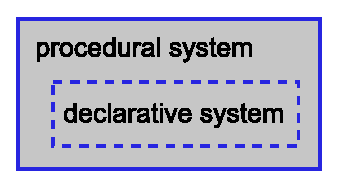
\includegraphics{Procedural-subsumes-Declarative-system.eps}
\end{figure}
\vspace{-0.5cm}

The procedural system communicates with the declarative system via various types of \textbf{querying}.  The declarative system itself has no means of performing actions;  its only function is question-answering.  There may be exceptions, but the general rule can be captured by the slogan \textit{``Procedural subsumes Declarative''}.

\section{The action language}
\label{sec:ActionLanguage}

We have represented declarative knowledge using a logical language; now we should represent procedural knowledge with a similar action language.

The following are examples of ``actions'':\\
1. say "hello"\\
2. open a file\\
3. print 1...100\\
4. repeat printing N until the user presses the Esc key

Do they sound like programming language tasks?  Thinking along this line, it seems advantageous that \textit{the action language should be a conventional programming language} such as C++, Java, Lisp,  Prolog, etc.

So the procedural system expresses actions in a programming language.  Those actions can be executed via the compiler or interpreter of that language.  In some situations, it is more convenient if the language can be interpreted.

The action output of the Procedural System can be of 3 forms:\\
1. a statement that is immediately interpreted and executed\\
2. a program that needs to be compiled\\
3. a program fragment that becomes part of the Procedural System

\#3 is actually a form of procedural learning.

\section{Procedural learning}
\label{sec:ProceduralLearning}

When the procedural language is complex, learning may be more difficult.  So there may be a need to restrict the procedural language.  %Secondly, there may be a need to put the learned procedures within a meta-controller framework so as to control them better.

Learned procedures can be inserted into the Procedural System at certain hook points.  Each hook point represents a context, for example ``We get here when the user presses the Esc key''.  The procedural learning algorithm should take such contexts into consideration.

``learn by being told'' is also applicable to procedural learning.

\section{Reinforcement learning} \index{reinforcement learning}
\label{sec:RL}

The goal of RL is to learn an optimal policy which is a function from the set of states to the set of actions:\\
\hspace*{1cm} $\pi: \mathbb{S} \rightarrow \mathbb{A}$.

RL can learn to:\\
1.  conversate with humans (eg in chat rooms)\\
2.  write programs\\
3.  crawl the web to learn things\\
and do all these without the need for human programming, so it is cost-effective.

See also \S\ref{sec:combine-DP-RL} on combining deductive planning and RL.

\subsection{Relational reinforcement learning}

(cf \citep*{Dzeroski1998}, \citep*{Dzeroski2001}, \citep*{Tadepalli2004}, \citep*{Driessens2005})

One problem with RL is that the number of states in a general intelligent agent is too large (in fact, infinite).  I suggest using FOL to describe the states so the formulation can be more compact.\\
A state would be a conjunction of ground literals, such as:\\
\hspace*{1cm} S1 = horny(john) $\wedge \; \neg$ good-looking(john) $\wedge$ has-money(john)\\
and the policy could be a rule that recommends an action from a state:\\
\hspace*{1cm} $\neg$ good-looking(X) $\wedge$ has-money(X) $\rightarrow$ try(X, buy-a-cybernetic-body)\\
Such a logical rule is not exactly a function, because:
\begin{compactenum}[1.]
\item More than one state can be true at the same time
\item If 2 states are both true and S2 $\supset$ S1, and\\
\hspace*{1cm} S1 $\rightarrow$ try(action1)\\
\hspace*{1cm} S2 $\rightarrow$ try(action2)\\
then both actions will be recommended when S2 is true.  We need a \textbf{conflict resolution} scheme to resolve this.\\
\{ TO-DO \} \\
\end{compactenum}

\subsection{RL and logical reasoning}

The relationship between RL and logical reasoning is very fascinating:  we can regard logical deduction as the task of searching for the proof of a query;  then RL can be used to perform deduction via learning the policy:\\
\hspace*{1cm} $\pi$ : search state $\mapsto$ search state.\\
From the previous section, we see that relational RL can vastly increase the expressive power of RL through generalization of states.  So the search states of the logical proof space can be generalized to what we call \textbf{cognitive states}, and the job of RL is to learn the policy:\\
\hspace*{1cm} $\pi$ : cognitive state $\mapsto$ cognitive state.

In this setting, the KB is part of the environment, and we'll have actions that manipulate the KB such as adding, subtracting, and searching KB items.

Thus, the entire logical reasoner can be implemented within RL.

The question now is how to represent cognitive states and their transitions.

\section{Means-ends analysis (MEA)}

MEA is a planning method proposed first by \citep*{Newell1960} for GPS (General Problem Solver).  They believed that MEA occurs in human problem solving.  It is  a \textit{forward} chaining feature-space\footnote{The feature space is similar to the state space except that a set of features only partially describe a state and thus can economically encompass many states.  This is a virtue in view of an agent's limited knowledge of the complex world.} search (ie, applying operators forwardly until the goal state is reached).  MEA selects a difference between the current state and the goal state, then selects an operator that may reduce the difference, and attempts to apply the operator.  If the operator's preconditions are not met, MEA recursively calls itself to transform the current state into one that meets those conditions.  If the conditions are met, MEA applies the operator and then recurse to transform the new state into the goal state (from \citep*{Langley1993}).

Wikipedia:  ``Note that, in order for MEA to be effective, the goal-seeking system must have a means of associating to any kind of detectable difference those actions that are relevant to reducing that difference.''

\{ TO-DO:  how to combine MEA with RL and deductive planning? \}

\section{Deductive planning}
\label{sec:deductive-planning}

A classical planning problem is represented by states and operators (actions).  Each operator has its precondition and effect.

In deductive planning based on situation calculus, actions are represented as terms, with the special predicates \code{do()} and \code{poss()}.

An advantage of deductive planning is that the Procedural System only needs to be an inference engine and nothing else.

One difficulty here is how to represent states, actions, preconditions, and effects;  especially actions.  I can put the cup on the table.  The current state is represented implicitly by all the facts in KB.  The actions are a special class of facts related to possibilities.  ``Water conducts electricity'' is a fact;  But ``water can conduct electricity'' is a possible action?  

Also, DP has a problem in that it only pursues one goal at a time.

\subsection{Example}

\begin{quote}
\emph{I try to kill Frank by tossing a radio in the bathtub while he is in it.  This may work because I know that water conducts electricity, and electricity can kill, etc.}
\end{quote}

Deductive planning allows the AGI to draw general knowledge from the KB to represent the planning problem:\\
\hspace*{1cm} goal = kill Frank\\
\hspace*{1cm} current state = Frank in bathtub, radio nearby\\
\hspace*{1cm} possible actions = toss radio into bathtub, slash Frank's wrist with a knife, etc\\
\hspace*{1cm} background knowledge = water conducts electricity, etc

\subsection{Combining reinforcement learning and deductive planning}
\label{sec:combine-DP-RL}

DP says:  ``If I do X, Y will probably happen as a result''.\\
RL says:  ``At state S, if I perform action A, the reward is probably high''.

We cannot simply have 2 planners co-existing -- the actions recommended by DP may conflict with those recommended by RL.  We may simply stipulate that the logical reasoner (since it is cognitively more sophisticated) has priority over RL.

RL may invoke DP for a recommendation of action.  When DP fails to find a recommendation, RL will act.

